%%%% using 'arara' 4.0
% arara: xelatex: {synctex: yes, interaction: nonstopmode}
% arara: bibtex
% arara: xelatex: {synctex: yes, interaction: nonstopmode}
% arara: xelatex: {synctex: yes, interaction: nonstopmode}

% arara: indent: {overwrite: yes}

% arara: clean: { extensions: [aux, bcf, cod, blg, lof, lot, out, toc, log, xml, bak0 ] }

\documentclass[review]{elsarticle}

% Figures Links, mittig und rechts platzieren
\usepackage[export]{adjustbox}
\usepackage{caption}
\usepackage{subcaption}
\usepackage{amsmath}

% prevents that appendices are moved behind references
\usepackage{placeins}

\usepackage[nolist]{acronym}

\usepackage{longtable}
\usepackage{booktabs}
\usepackage{multirow}
\usepackage{float}

\graphicspath{{../03_figures/results/}{./}{../03_figures/data/}} 

% enable paragraph as 4th level https://tex.stackexchange.com/questions/60209/how-to-add-an-extra-level-of-sections-with-headings-below-subsubsection
\usepackage{titlesec}
\setcounter{secnumdepth}{4}
\titleformat{\paragraph}
{\normalfont\small\bfseries}{\theparagraph}{1em}{}
\titlespacing*{\paragraph}
{0pt}{3.25ex plus 1ex minus .2ex}{1.5ex plus .2ex}

% enable linking to subsubsection
\setcounter{secnumdepth}{3}

% various symbols, e.g. \degree
\usepackage{gensymb}

\usepackage[hidelinks]{hyperref}

\usepackage{lineno}
\modulolinenumbers[5]

% set autoref abbr for appendix
\newcommand*{\Appendixautorefname}{appendix}

\journal{Journal "Remote Sensing of Environment"}

% line breaks in table cells
\newcommand{\specialcell}[2][l]{%
  \begin{tabular}[#1]{@{}l@{}}#2\end{tabular}}

% tilde
\newcommand{\mytilde}{\raise.17ex\hbox{$\scriptstyle\mathtt{\sim}$}}

%% APA style
\bibliographystyle{model5-names}\biboptions{authoryear}

\begin{document}

\begin{frontmatter}

	\title{title}

	%% Group authors per affiliation:
	\author[FSU]{Patrick Schratz}
	\cortext[mycorrespondingauthor]{Corresponding author}
	\ead{patrick.schratz@uni-jena.de}

	\author[FSU]{Jannes Muenchow}
	\author[NEIKER]{Eugenia Iturritxa}
	%\author[TUDO]{Jakob Richter}
	\author[FSU]{Alexander Brenning}

	\address[FSU]{Department of Geography, GIScience group, Grietgasse 6, 07743, Jena, Germany}
	%\address[NEIKER]{NEIKER, Granja Modelo –Arkaute, Apdo. 46, 01080 Vitoria-Gasteiz, Arab, Spain}
	%\address[TUDO]{Department of Statistics, TU Dortmund University, Germany}

	\begin{abstract}

	\end{abstract}

	\begin{keyword}
		hyperspectral imagery \sep forest health \sep machine-learning \sep variable importance \sep model comparison
	\end{keyword}

\end{frontmatter}

\linenumbers

% längste Abkürzung steht hier!!! in eckigen Klammern
\begin{acronym}[AUROC]

	% geringerer Zeilenabstand
	%\setlength{\itemsep}{-\parsep}
	\acro{AGB}{Above-Ground Biomass}
	\acro{ANN}{Artificial Neural Network}
	\acro{AUROC}{Area Under the Receiver Operating Characteristics Curve}
	\acro{BRT}{Boosted Regression Trees}
	\acro{CART}{Classification and Regression Trees}
	\acro{CV}{cross-validation}
	\acro{ENM}{Environmental Niche Modeling}
	\acro{FPR}{False Positive Rate}
	\acro{GAM}{Generalized Additive Model}
	\acro{GBM}{Gradient Boosting Machine}
	\acro{GLM}{Generalized Linear Model}
	\acro{ICGC}{Institut Cartografic i Geologic de Catalunya}
	\acro{IQR}{Interquartile Range}
	\acro{WKNN}{Weighted $k$-nearest neighbor}
	\acro{MARS}{Multivariate Adaptive Regression Splines}
	\acro{MEM}{Maximum Entropy Model}
	\acro{NRI}{Normalized Ratio Indeces}
	\acro{OLS}{Ordinary Least Squares}
	\acro{LOWESS}{Locally Weighted Scatter Plot Smoothing}
	\acro{PISR}{Potential Incoming Solar Radiation}
	\acro{RBF}{Radial Basis Function}
	\acro{RF}{Random Forest}
	\acro{RMSE}{Root Mean Square Error}
	\acro{RR}{Ridge Regression}
	\acro{RSS}{Residual Sum of Squares}
	\acro{SDM}{Species Distribution Modeling}
	\acro{SMBO}{Sequential-based Model Optimization}
	\acro{SVM}{Support Vector Machines}
	\acro{TPR}{True Positive Rate}
\end{acronym}

\section{Introduction}
\label{sec:intro}

% Explain how remote sensing is used in forestry (potential to map forest health)
Remote sensing data is successfully used in forestry to monitor temporal changes across large areas REFERENCES.
The use of SAR techniques enables scientists to estimate \ac{AGB}.
Forest health is commonly modelled using optical data from multispectral satellites by applying temporal change detections.
With a well-trained model, scientists are able to predict the modelled response to a large area, giving valuable information about the environmental condition of this region.
To model forest health, usually vegetation indices are derived from the band values, i.e. band combinations that are proven to be sensitive to health changes of vegetation.
However, the pool of possible indices is often limited due to a low spectral resolution of freely available data from multispectral sensors.
Also, if the spatial resolution of the data is too coarse (e.g. > 5 m), the value of a pixel contains information of multiple trees and possibly even bare-ground information.
These problems introduce bias into the data which is passed onto the fitted model, leading to non-optimal modeling results.

% Why are we mapping defoliation?

In this study we will use hyperspectral remote sensing data with a spatial resolution of one meter and 126 spectral bands to model defoliation of \textit{Pinus radiata} trees in northern Spain. 
These trees suffer from infections of invasive pathogens such as \textit{Diplodia sapinea}, \textit{Armillaria} or \textit{Heterobasidion} leading to a spread of cankers or defoliation before the tree dies.
The fungis are assumed to infect the trees through open wounds, possibly caused by hail damage \citep{Iturritxa2014}.
The dieback of these trees, which are mainly used as timber, causes high economic damages in the Iberian Peninsula area.
Remote sensing data in combination with state-of-the-art machine-learning techniques can help to constantly monitor forest health in this region using proxies such as defoliation of the tree crown.
With this information, an increase in defoliation can serve as an early-warning indicator of a possible infection of a plot.

% Show importance of vegetation indices and NRI

To extract the most information from the available remote sensing data, we not only calculated the most often used vegetation indices (e.g. NDVI) to link against defoliation. 
The narrow bands of the given data enable the calculation of up to 90 vegetation indices.
Additionally, all possible combinations of \ac{NRI} were calculated from the data and supplied to the machine-learning algorithms as predictors.
With their ability to find patterns between the response and its predictors in the data, we hope to increase the predictive accuracy of defoliation based on remote sensing indices.

% Mention the ability of ML algs to handle highly correlated variables

In this study the following objectives are addressed: 

\begin{itemize}
	\item Checking multiple machine-learning algorithms on their ability to model defoliation of \textit{Pinus radiata} trees
	\item Exploration of the most important indices of the model
	\item Prediction of defoliation to plots with unknown levels of defoliation
\end{itemize}

\section{Data and study area}

\subsection{In-situ data}
% Describe Plots

The \textit{Pinus radiata} plots of this study, named \textit{Laukiz 1}, \textit{Laukiz 2}, \textit{Luiando} and \textit{Oiartzun}, are located in the northern part of the Basque Country (\autoref{fig:study_area}).
\textit{Oiartzun} has the most observations (n = 529) while \textit{Laukiz 2} has the largest area size (1.44 ha).
All plots besides \textit{Luiando} are located nearby the coast (\autoref{fig:study_area}).
The data collection took place in September 2016.

\begin{figure} [t!]
	\begin{center}
		\makebox[\textwidth]{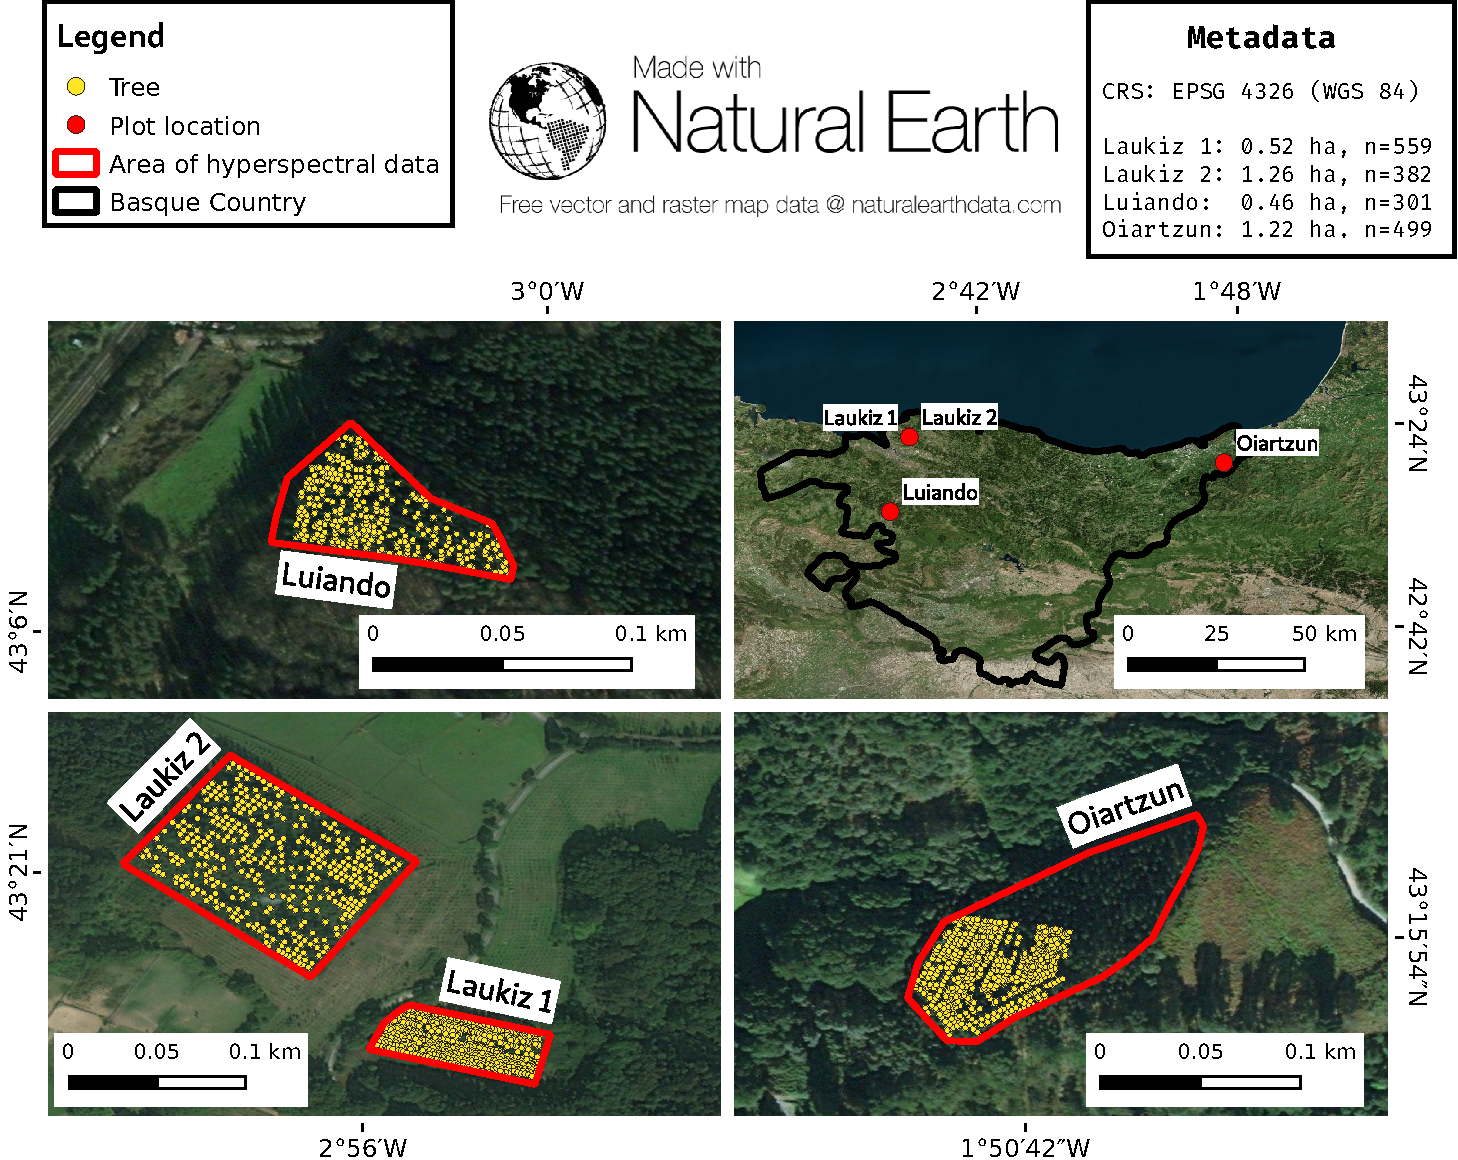
\includegraphics[width=\textwidth] {study_area_hyperspectral.pdf}}
		\caption{Information about the plot locations, the area of hyperspectral coverage and the number of trees per plot.}
		\label{fig:study_area}
	\end{center}
\end{figure}

\subsection{Hyperspectral data}

The airborne hyperspectral data was acquired during two flight campaigns on September 28th and October 5th 2016, both around 12 am.
The images were taken by an AISAEAGLE-II sensor from the \ac{ICGC}.
All preprocessing steps (geometric, radiometric, atmospheric) have been conducted by \ac{ICGC}.
The first four bands were corrupted, leaving 122 bands with valid information.

Additional data characteristics are provided in Table 1:

% parameter limits
\begin{table}[b!]
\centering
\caption[t]{Specifications of hyperspectral data.}
\begingroup\footnotesize
\begin{tabular}{ll}
	\\
	Characteristic         & Value                               \\
	\hline
	Geometric resolution   & 1 m                                 \\
	Radiometric resolution & 12 bit                              \\
	Spectral resolution    & 126 bands (404.08 nm - 996.31 nm)   \\
	Correction:            & Radiometric, geometric, atmospheric
\end{tabular}
\endgroup
\label{tab:hyperparameter_limits}
\end{table}

\section{Methods}

For all analysis steps we used the open-source statistical programming language R \citep{R_core}.
The algorithm implementations of the following packages have been used: \textit{xgboost} \citep{chenXGBoostScalableTree2016}, \textit{kernlab} \citep{kernlab} (Support Vector Machine), \cite{Vapnik1998}) and \textit{glmnet} \citep{glmnet} (Ridge Regression). 
We used the R package \textit{mlr} for all modeling related steps.
It provides a standardized interface for a wide variety of statistical and machine-learning models in R simplifying essential modeling tasks such as hyperparameter tuning, model performance evaluation and parallelization \citep{bischlMlrMachineLearning2016}.

\subsection{Derivation of indices}

% link to PDF with veg indices
All vegetation indices (90 total) suitable for the wavelength range of the hyperspectral data that were available in the R package \textit{hsdar} have been calculated.
Additionally, all possible \ac{NRI} were calculated from the data using the formula:

\begin{equation}
	NRI_{i,j} = \frac{b_{i} - b_{j}}{b_{i} + b_{j}}
\end{equation}

\noindent
where $i$ and $j$ are the respective band numbers.

%To account for geometric offsets, we calculated every index five times using a buffer from 1 - 5 meter around the centroid of the respective tree.
To account for geometric offsets, we used a buffer of two meters around the centroid of the respective tree.
The mean value of all pixels touched by the buffer was assigned as the final value for each index.
Missing values were removed from the mean value calculation.
In total, 7875 Normalized Ratio Indices NRI have been calculated ($\frac{125*126}{2}$).
Due to four corrupted bands and some other numerical problems, few indices returned \texttt{NA} values for some observations.
These indices were removed from the dataset, leaving a total of 7471 variables without missing values.

\subsection{Exploratory analysis of plot characteristics}

Plot characteristics like age, stand density and defoliation were analysed to show differences among the plots.
Additionally, the spectral signatures of each plot have been visualized. 

\subsection{Benchmarking of algorithms}

Multiple algorithms were benchmarked on predictive performance to find the best performing one.
Besides the well-known \ac{SVM} \citep{Vapnik1998} we also used \textit{xgboost} which is ensemble method relying on the idea of tree boosting that gained a lot of attention in recent years \citep{chenXGBoostScalableTree2016}.
We also added penalized L2 (Ridge) regression to the algorithm collection due to its ability to handle highly correlated covariates.
We also want to explain why we did not consider the probably most popular machine-learning algorithm, Random Forest: Due to the high number of variables model fitting times in the range hours for a single model fit were not practicable for this work. 
These high fitting times are caused by hyperparameter \texttt{mtry} which scales with the number of variables \citep{Probst2018b}.

% \subsubsection{The ridge penalty}

% In \ac{RR} (also called $\ell_{2}$ penalization) the assumption of unbiased coefficients is given up in favor of higher predictive accuracy and reduced variance \citep{Hastie2001}.
% Coefficients are standardized and penalized for their size.
% When minimizing the \ac{RSS}, \ac{RR} adds a penalization term $\lambda \sum_{j=1}^{p}\beta_{j}^{2}$ to the equation:

% \begin{equation}
% 	RSS = \sum_{i=1}^{n} \left(y_{i} - \beta_{0} - \sum_{j=1}^{p} \beta_{j} x_{ij} \right) ^{2} + \lambda \sum_{j=1}^{p}\beta_{j}^{2}
% \end{equation}

% where $\lambda >= 0$ is a tuning parameter responsible for the magnitude of penalization.
% To make the second term (usually referred to as the \textit{shrinkage penalty}) of this equation small, the coefficients $\beta_{j}$ need to become small.
% Unlike to Lasso however, predictors are not removed from the final model and will always be $\beta_{j} >= 0$.
% Hence, $\lambda$ has the effect of shrinking the coefficients when minimizing the \ac{RSS}.
% For $\lambda = 0$, no penalization is done and standard \ac{OLS} applies \citep{James2013}.
% The \textit{shrinkage penalty} is only applied to the coefficients and not to the intercept.
% Also, while \ac{OLS} generates only one set of coefficient estimates, \ac{RR} will create multiple sets for every value of $\lambda$.
% In summary, the advantage of \ac{RR} is based on the bias-variance tradeoff: For $\lambda\to\infty$, the flexibility of the fit is reduced leading to a decrease in variance of the coefficients but also introduces a (substantial) bias.
% For $\lambda = 0$, the variance is high but coefficients are unbiased \citep{James2013}.

\subsubsection{Performance estimation}

The algorithms were benchmarked in two ways: 
(1) Using spatial \ac{CV} for each plot using on the k-means clustering approach of \cite{Brenning2012}. To reduce runtime we used a five-fold five-times repeated CV setup.
(2) Using spatial \ac{CV} on the plot level with each plot being the test set once. This results in four performance estimates, one for each fold.
For (1) we only used the best performing algorithm from (2). 
The reason why the (2) was chosen for algorithm selection is that this model will also be used to spatially predict defoliation in other plots.

% Add figure visualizing both spCV approaches

\subsubsection{Hyperparameter tuning}
To tune the hyperparameters of the algorithms, we used \ac{SMBO} via the R package \textit{mlrMBO} \citep{mlrMBO}.
This Bayesian approach first composes \textit{n} randomly chosen hyperparameter settings out of a user defined search space.
After these \textit{n} tries have been evaluated, a new hyperparameter setting to be evaluated next is proposed based on the setting that performed best.
This strategy continues until a termination criterion, defined by the user, is reached \citep{Hutter2011, Jones1998}.
In this work we used an initial design of 30 randomly composed hyperparameter settings and a termination criterion of 20 iterations, resulting a total budget of 50 evaluated hyperparameter settings per fold.
The advantage of this tuning approach is that it substantially reduces the tuning budget which is needed to find a setting close to the global minimum compared to methods that do not use information from previous runs such as \textit{random search} or \textit{grid search} \citep{Bergstra2012}.

\subsection{Variable importance}

To find indices that contributed most to model performance, we used permutation-based variable importance on the best performing algorithm.

% partial dependence plots??

\section{Results}

\subsection{Exploratory data analysis}

% defoliation boxplots
\begin{figure} [t!]
	\begin{center}
		\makebox[\textwidth]{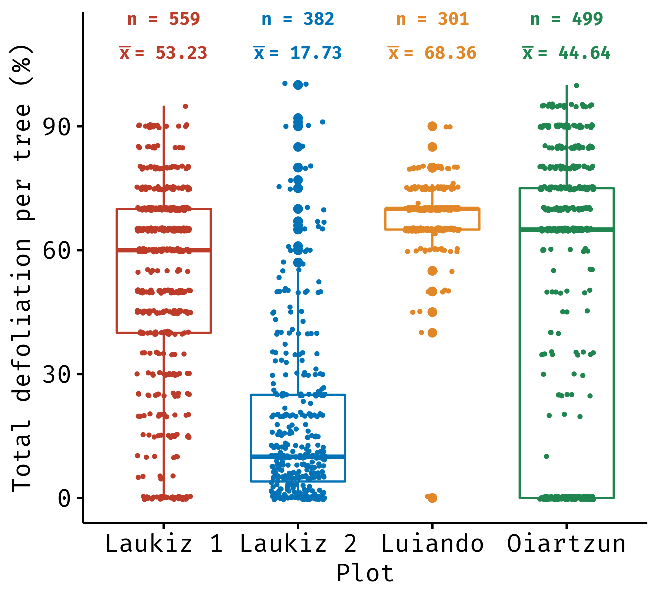
\includegraphics[width=0.7\textwidth] {boxplot_defol.pdf}}
		\caption{Descriptive statistics of the response variable \textit{defoliation}.}
		\label{fig:defol_boxplots}
	\end{center}
\end{figure}

% spectral signatures
\begin{figure} [t!]
	\begin{center}
		\makebox[\textwidth]{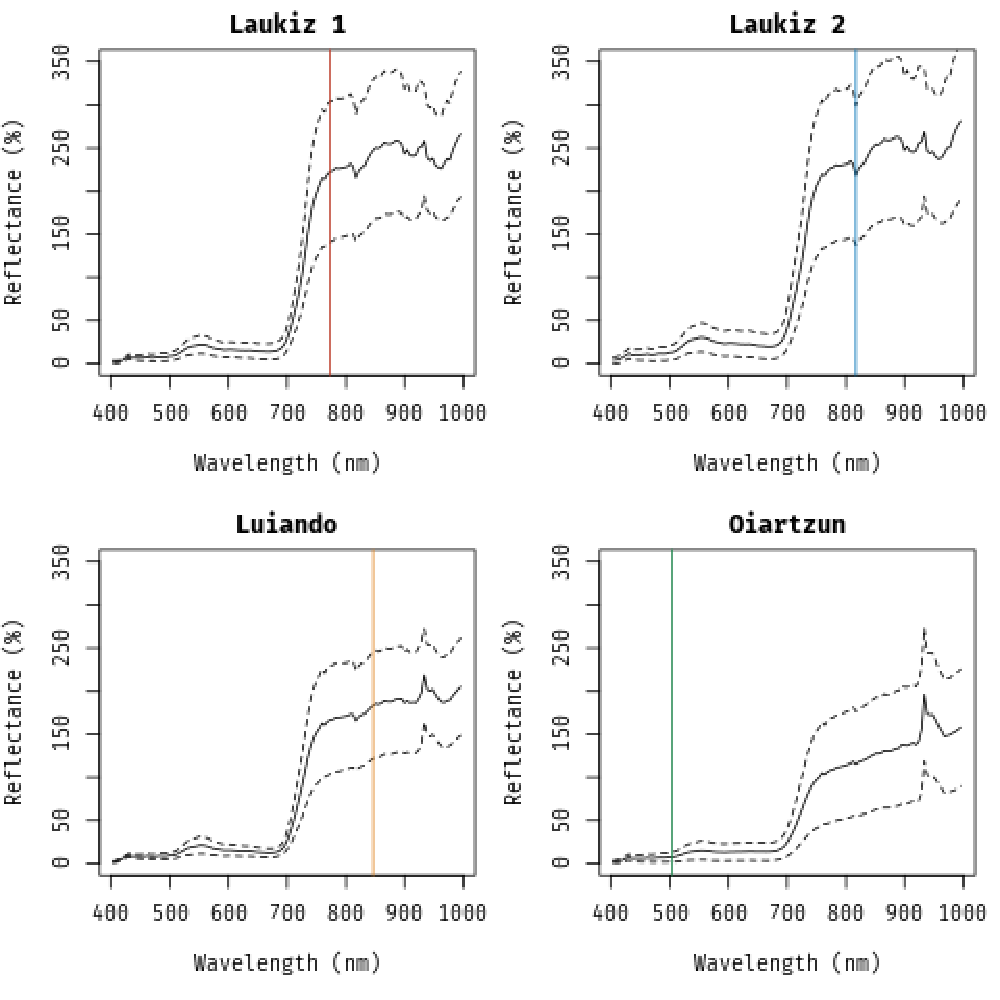
\includegraphics[width=\textwidth] {spectral_signatures.pdf}}
		\caption{Spectral signatures (mean and standard deviation) of each plot.
			The colored lines show the most important band for each plot, respectively: Band 80 (773nm, red), band 89 (817nm, blue), band 95 (846nm, orange), band 23 (503nm, green).}
		\label{fig:spectral_signatures}
	\end{center}
\end{figure}

\textit{Oiartzun} shows the highest defoliation ($\bar{x} = 69.22 \%$) among the plots while \textit{Laukiz 2} is the healthiest ($\bar{x} = 13.54 \%$) (\autoref{fig:defol_boxplots}).
All plots besides \textit{Luiando} show an evenly distributed level of defoliation across the entire plot.

The high degree of defoliation of \textit{Luiando} and \textit{Oiartzun} is also visible in the spectral signatures of the plots (\autoref{fig:spectral_signatures}).
Both plots show lower mean reflectance values around the wavelength range 800 nm - 1000 nm compared to Laukiz 1 and Laukiz 2.
Oiartzun is almost completely missing the reflectance drop at around 815 nm that is visible for all other plots but instead shows a higher magnitude for the reflectance increase at around 920 nm.
Laukiz 2 shows a mean tree density of 61.59 m \autoref{fig:rmse_defol_dens}) while all other plots are more dense (34.64 (Laukiz 1), 33.01 (Luiando), 34.96 (Oiartzun)) (\autoref{fig:plot-characteristics}).

\subsection{Predictive performance}

% Performance estimates
\begin{table}[b!]
	\centering
	\caption[t]{Four-fold spatial \ac{CV} performances of RR, SVM and xgboost using \ac{RMSE} as the error measure. 
	Mean and standard deviation are shown.}
	\begingroup\footnotesize
	\begin{tabular}{llll}
		RR            & SVM           & xgboost \\
		\hline
		59.10 (22.71) & 36.23 (15.73) &  &         \\
		\bottomrule
	\end{tabular}
	\endgroup
	\label{tab:penalty_comparison}
	\end{table}

\begin{table}[t!]
\centering
\caption[t]{Predictive performance of xgboost using the merged dataset (supermodel) and observations on a plot level only (single plot) with \ac{RMSE} as the error measure. The performance estimates for "All Plots" correspond to the fold for which the respective plot was serving as the test set. For "single plot", the values correspond to the mean value of the SpCV at the repetition level (10 folds, 20 repetitions), scored by models fitted on the data of the respective plot only.}
\begingroup\footnotesize
\begin{tabular}{lll}
	\\
	Plot/Data & All Plots (Block CV) & Single plot (SpCV) \\
	\hline
	Laukiz 1  & 58.95                     & 89.89              \\
	Laukiz 2  & 27.94                     & 30.37              \\
	Luiando   & 69.72                     & 76.02              \\
	Oiartzun  & 58.09                     & 106.65             \\ 
	\bottomrule
\end{tabular}
\endgroup
\label{tab:supermodel_performance}
\end{table}

\ac{RR} shows the lowest error for three out of four plots (for Luiando \textit{elasticnet} shows a slightly better performance) (\autoref{tab:penalty_comparison}).
The magnitude of difference for \ac{RR} compared to the other penalties for the plots in which \ac{RR} showed the best performance ranges between XX and XX percent.
For the merged dataset, all penalties show a similar mean predictive performance that outperform all single plot models besides the Laukiz 2 model.

% single models vs supermodel
When comparing the mean predictive performance of the plot level model against the performance of the super model at the plot level (when the respective plot served as the test set), the supermodel also outperforms the Laukiz 2 model (27.94 vs 30.37 RMSE) (\autoref{tab:supermodel_performance}).

The worst performance of the supermodel on the fold level is reported for Luiando (69.72 RMSE) while for the single plot models Oiartzun shows the highest error (106.65 RMSE).

% RMSE vs CV and point dens
Laukiz 2 showed contrary results compared to all other plots when linking \ac{RMSE} against coefficient of variation and mean point density (\autoref{fig:rmse_defol_dens}).
Comparing RMSE against $CV/skewness$ shows a $log_{2}(-x)$ relationship.

% rmse vs defol and point dens
\begin{figure} [b!]
	\begin{center}
		\makebox[\textwidth]{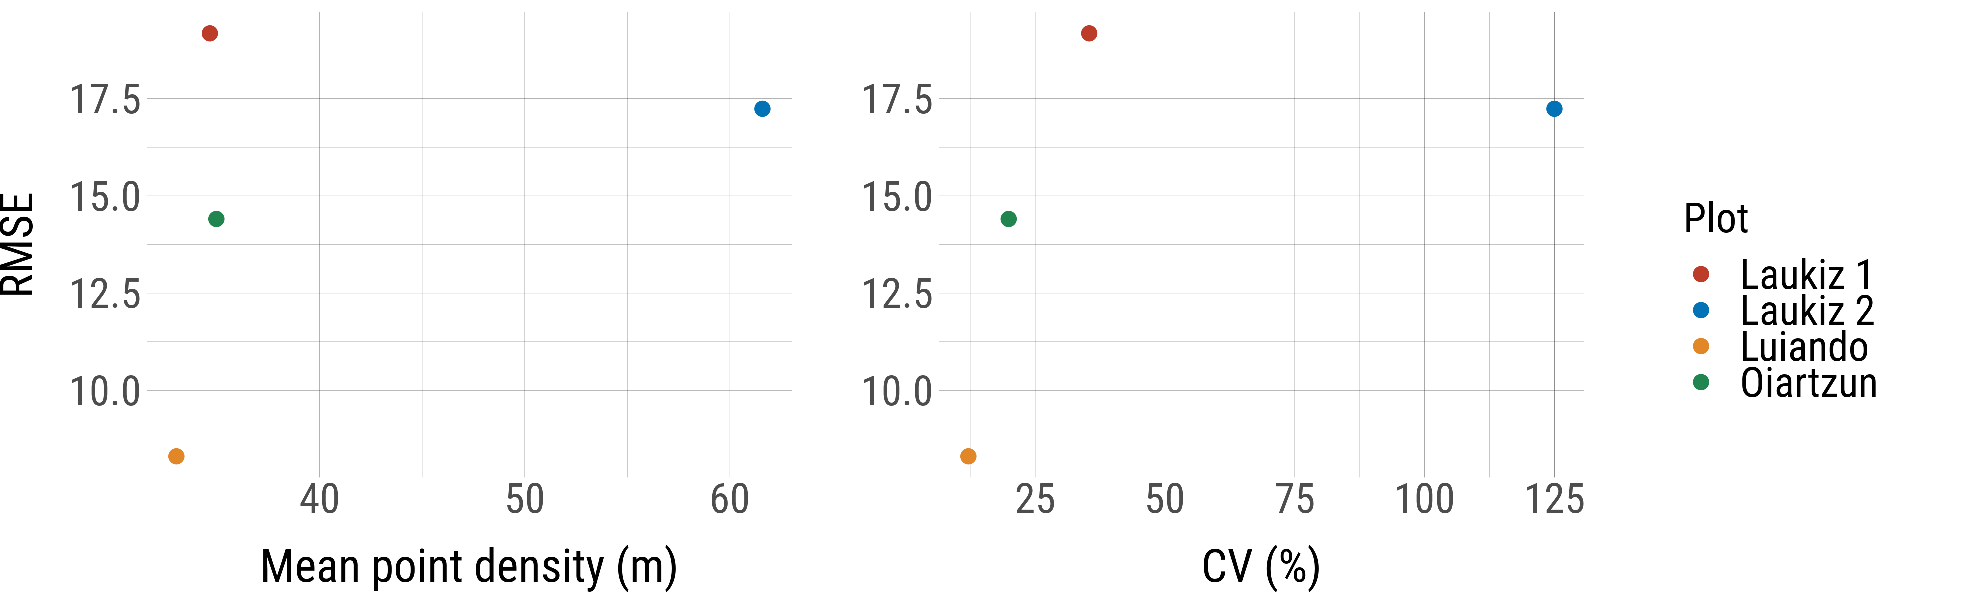
\includegraphics[width=\textwidth] {../03_figures/results/plot-characteristics.pdf}}
		\caption{RMSE vs. mean point density, coefficient of variation and coefficient of variation / skewness.}
		\label{fig:plot-characteristics}
	\end{center}
\end{figure}

\subsubsection{Variable importance}

\ac{NRI}s using bands in the wavelength range of 770 nm - 820 nm (band 80 - band 89), which belongs to the infrared region, appear most often among the ten highest coefficient estimates across all plots (\autoref{tab:variable-importance}).
Only one vegeation index (Datt3) showed up among the most important predictors (Laukiz 1).
Luiando and Oiartzun also prefered bands with longer (938.39 nm (band 114) - 996.31 nm (band 126)) and shorter wavelengths (480.30 nm (band 18) - 503.26 (band 23)).
The first range again belongs to the infrared region while the second is within the region of the visible light, transitioning from blue to green.


% band importance
\begin{figure} [b!]
	\begin{center}
		\makebox[\textwidth]{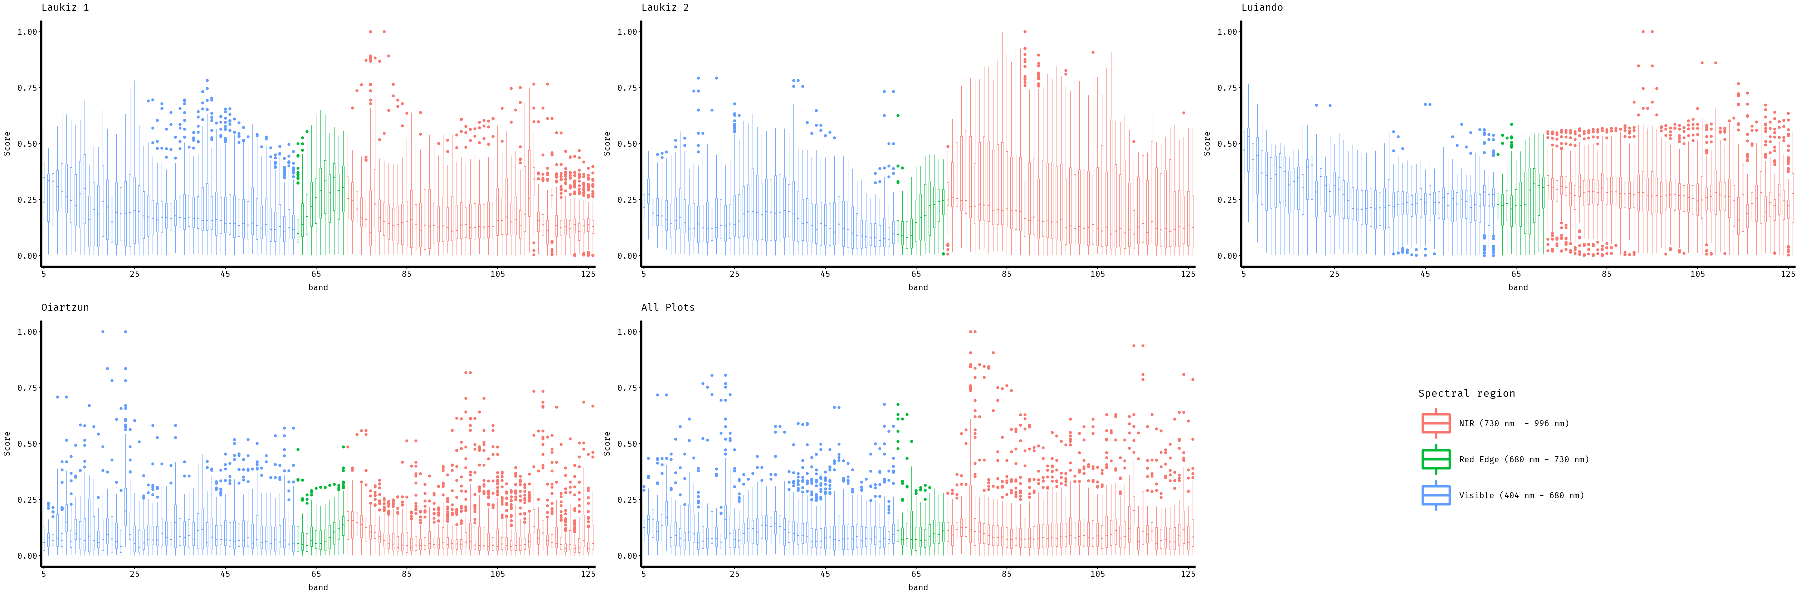
\includegraphics[angle=90, height = 0.95\textheight] {../03_figures/results/important-bands_boxplot.pdf}}
		\caption{test}
		\label{fig:important-bands}
	\end{center}
\end{figure}

\section{Discussion}

\subsection{Index derivation}

The exact number of contributing pixels to the final index value of an observations cannot be determined as it depends on the location of the tree within the pixel grid.
If a tree is located at the border of a pixel, a buffer of e.g. three meters will include more pixels than if the point is located at the center of a pixel.
Also, if a tree is located at the border of the plot, some directions of the buffer will not contain image values.

\subsection{Plot characteristics}

For Laukiz1, Luiando and Oiartzun \ac{RMSE} seems to increase with a higher point density at a first glance.
However, the point densities of these plots are very similar (33.7 m - 35.01 m) and should be interpreted as a group instead of single values.
With Laukiz2 being completely off from the other plots in terms of mean point density, no pattern can be extracted from this result.
Linking RMSE vs coefficient of variation shows the same relationship as linking against mean point density.
The interesting $log_{2}(-x)$ relationship for RMSE vs. coefficient of variation / skewness should be interpreted with caution: The sample size of four plots is not representative to make general statements here.
This finding should be verified with more observations in future studies.

\subsection{Variable importance}


\section*{References}

\bibliography{Biblio_hyperspectral}

\end{document}
